\documentclass[11pt]{article}

\usepackage[margin=1in]{geometry}
\usepackage{times}
\usepackage{graphicx}
\usepackage{hyperref}
\usepackage{xcolor}
\usepackage{booktabs}
\usepackage{array}
\usepackage{enumitem}
\usepackage{listings}
\usepackage{caption}
\usepackage{float}

\hypersetup{
    colorlinks=true,
    linkcolor=blue,
    citecolor=blue,
    urlcolor=blue
}

\lstdefinestyle{code}{
    basicstyle=\ttfamily\small,
    breaklines=true,
    frame=single,
    columns=fullflexible,
    backgroundcolor=\color{gray!6},
    rulecolor=\color{gray!40}
}
\lstset{style=code}

\setlist[itemize]{leftmargin=1.5em}
\setlist[enumerate]{leftmargin=1.5em}

\title{\textbf{Project Proposal: SAMBA-Inspired Sparsity-Aware In-Memory Computing Accelerator Simulator}}
\author{Hanuman Ashik Akshintala\\Course Project Proposal}
\date{}

\begin{document}

\maketitle

\section{Introduction}

This project is based on the paper ``SAMBA: Sparsity Aware In-Memory Computing Based Machine Learning Accelerator'' by Kim, Ankit, Wang, and Roy. The paper studies a machine-learning accelerator that uses analog in-memory computing (IMC) to reduce the cost of data movement during neural-network inference. In analog IMC, matrix-vector multiplication can be performed directly inside memory crossbar arrays, instead of repeatedly moving weights between memory and a processor.

The important bottleneck in this type of accelerator is the analog-to-digital converter (ADC). The crossbar produces analog outputs, but the rest of the system must consume digital values. Therefore, ADCs are required after crossbar computation. ADC cost grows with precision, so high-precision ADCs can dominate latency and energy.

The SAMBA paper proposes to use sparsity in machine-learning weights to reduce ADC precision and improve inference efficiency. Many neural-network weights become zero after pruning. If a crossbar column has many zeros, then the output range is smaller and the ADC can use fewer bits. However, sparsity is often uneven. Some crossbars may be highly sparse, while others may be dense. Because multiple MVMUs execute together, one slow dense block can become the bottleneck. SAMBA addresses this by using load balancing and better data-movement scheduling.

In this project, I propose to build a software simulator for a SAMBA-style sparsity-aware analog IMC accelerator. The simulator will compare a fixed-ADC PUMA-style baseline, a sparse reconfigurable-ADC baseline, and a SAMBA-style optimized design. The project will focus on architectural modeling, workload mapping, ADC precision estimation, load balancing, data movement, and performance reporting.

The goal is not to fabricate hardware or reproduce transistor-level circuit behavior. Instead, the goal is to build a reproducible architectural simulator that can explain why SAMBA-style optimizations improve latency and energy efficiency.

\section{Method}

The proposed system is a Python-based accelerator simulator. The high-level project workflow is:

\begin{center}
\texttt{Neural Network Weights $\rightarrow$ Crossbar Mapping $\rightarrow$ ADC Model $\rightarrow$ SAMBA Optimizations $\rightarrow$ Results Dashboard}
\end{center}

\subsection{Planned System Components}

\begin{itemize}
    \item \textbf{Workload Generator:} Generate synthetic convolutional and fully connected layers with controllable sparsity. The final version will include VGG19-style and ResNet50-style workloads.
    \item \textbf{Crossbar Mapper:} Partition neural-network weight matrices into crossbar-sized matrix-vector multiplication units (MVMUs).
    \item \textbf{ADC Cost Model:} Estimate ADC precision, latency, and energy using the sparsity of each bit-sliced crossbar column.
    \item \textbf{Intra-Matrix Load Balancer:} Implement column exchange and row exchange to reduce uneven sparsity across MVMUs.
    \item \textbf{Inter-Matrix Load Balancer:} Implement split MVMU mapping for slow dense blocks.
    \item \textbf{Data-Movement Scheduler:} Compare baseline chain reduction with optimized tree/sort scheduling and input prefetching.
    \item \textbf{Experiment Runner:} Run controlled comparisons across baselines, SAMBA components, and hardware configurations.
    \item \textbf{React/Material UI Dashboard:} Present the final results using a clean dashboard with speedup, energy, ablation, and layer-bottleneck views.
\end{itemize}

\subsection{Baseline and Proposed Designs}

The simulator will compare three main accelerator modes:

\begin{itemize}
    \item \textbf{Fixed ADC Baseline:} A PUMA-style analog IMC baseline where every ADC uses fixed precision.
    \item \textbf{Sparse ADC Baseline:} A baseline that lowers ADC precision based on static weight sparsity but does not perform SAMBA load balancing.
    \item \textbf{SAMBA-Style Design:} A design that combines sparse ADC precision, load balancing, and optimized data movement.
\end{itemize}

\subsection{ADC Precision Model}

The simulator will model weights as fixed-point values partitioned into bit slices. For each crossbar column, the required ADC precision will be estimated from the possible accumulated output range. Sparse columns should require fewer ADC bits, while dense columns require more bits.

The simulator will track:

\begin{itemize}
    \item required ADC precision per column,
    \item MVMU latency,
    \item ADC energy,
    \item shift-and-add cost,
    \item data movement cost,
    \item load-balancing overhead.
\end{itemize}

\subsection{SAMBA Optimizations to Implement}

The planned SAMBA-style optimizations are:

\begin{itemize}
    \item \textbf{Column Exchange:} Swap high-cost columns from slow MVMUs with low-cost columns from faster MVMUs.
    \item \textbf{Row Exchange:} Swap rows across row-block groups to balance input-side sparsity.
    \item \textbf{Split MVMU:} Split slow dense MVMUs into two parallel MVMUs and merge their results.
    \item \textbf{Optimized Allocation:} Allocate MVMUs to cores in a way that reduces expensive inter-core rearrangement.
    \item \textbf{Tree Reduction and Sorting:} Reduce partial sums using a latency-aware tree instead of a simple chain.
    \item \textbf{Input Prefetching:} Model earlier loading of future convolution inputs to reduce idle time.
\end{itemize}

\subsection{Critical and Interesting Points}

The critical part of this project is not only to show that sparse ADC helps, but also to show why sparse ADC alone is not enough. If one dense MVMU is mapped with sparse MVMUs, the dense MVMU can determine the whole core latency. Therefore, the simulator must model bottlenecks, not only average sparsity.

Another important point is that load balancing is not always free. Column exchange and row exchange can require rearrange operations. Split MVMUs can require extra merge operations. Therefore, the final simulator should include overheads and compare whether an optimization is actually profitable.

\section{Parameters and Experiments}

The final evaluation will compare both workloads and hardware settings.

\subsection{Workloads}

\begin{itemize}
    \item Small microbenchmarks with balanced and unbalanced sparsity.
    \item VGG19-style convolutional workloads.
    \item ResNet50-style convolutional workloads.
\end{itemize}

\subsection{Hardware Parameters}

\begin{itemize}
    \item Crossbar size: 16, 32, and 64.
    \item Weight precision: 8-bit and 16-bit fixed-point settings.
    \item Bits per weight slice: 1-bit and 2-bit settings.
    \item MVMUs per core: 2, 4, 8, and 16.
    \item Cores per tile: 2, 4, and 8.
\end{itemize}

\subsection{Optimization Variants}

The final experiments will compare:

\begin{itemize}
    \item fixed ADC baseline,
    \item sparse ADC baseline,
    \item column exchange only,
    \item row exchange only,
    \item split MVMU only,
    \item data movement optimization only,
    \item full SAMBA-style optimization.
\end{itemize}

\subsection{Metrics}

The main metrics will be:

\begin{itemize}
    \item total latency cycles,
    \item total estimated energy,
    \item speedup over fixed ADC baseline,
    \item energy-efficiency improvement over fixed ADC baseline,
    \item layer-level bottlenecks,
    \item core utilization,
    \item data movement cycles,
    \item number of load-balancing operations.
\end{itemize}

\section{Use of Large Language Models}

I used ChatGPT as a support tool while working on this project. After reading the SAMBA paper, I used it to check my understanding of the main architecture ideas, especially analog in-memory computing, reconfigurable ADC precision, sparsity-aware weight mapping, MVMU load balancing, and data movement across cores and tiles.

During the preliminary implementation, I used it mainly when I ran into modeling, coding, and debugging issues. For example, I asked questions about how to structure a Python-based accelerator simulator, how to calculate ADC precision from sparse crossbar columns, and how to organize experiment outputs. I still reviewed the suggestions and tested the changes myself.

For the output display, I first generated simple JSON, CSV, and Markdown reports from the simulator results. After that, I used ChatGPT to help make the output cleaner by planning a React dashboard using Material UI for speedup, energy, ablation, and layer-bottleneck results.

Example prompts used during development included:

\begin{quote}
After reading the paper ``SAMBA: Sparsity Aware In-Memory Computing Based Machine Learning Accelerator,'' explain the main architecture ideas related to analog in-memory computing, ADC precision, sparsity, load balancing, and data movement.
\end{quote}

\begin{quote}
I am implementing a local Python simulator for a SAMBA-style analog IMC accelerator. Help me debug issues in the crossbar mapping and ADC precision calculation.
\end{quote}

\begin{quote}
My simulator is producing latency and energy numbers for fixed ADC, sparse ADC, and SAMBA-style optimization. Help me identify checks I can use to verify that the comparison is fair.
\end{quote}

\begin{quote}
I have basic JSON, CSV, and Markdown reports showing latency, energy, speedup, and layer bottlenecks. Help me redesign the output as a cleaner React dashboard using Material UI.
\end{quote}

The prompts were improved during development by making them more specific. For example, instead of asking only for general help with the paper, I added the exact simulator components I was using, such as crossbar MVMUs, ADC bit precision, sparse weight mapping, load balancing, VGG19/ResNet50-style workloads, latency and energy metrics, and the dashboard output. This made the responses more useful for debugging and presentation improvements.

\section{Preliminary Progress}

The current work is preliminary and is included only to show feasibility. I have started building a local simulator structure and small experiment pipeline. The preliminary prototype can generate sparse synthetic layers, map weights to crossbar blocks, estimate ADC cost, and produce basic result files.

The final numbers are not complete yet. For the final report, I will run larger workloads, complete the ablation study, and add a polished React/Material UI dashboard.

\subsection{Preliminary Prototype Output}

One early microbenchmark run compares fixed ADC, sparse ADC, and a preliminary SAMBA-style configuration. The purpose of this result is to show that the simulator can run end-to-end, not to claim final performance.

\begin{table}[H]
\centering
\caption{Preliminary microbenchmark result.}
\begin{tabular}{lrrr}
\toprule
\textbf{Design} & \textbf{Latency Cycles} & \textbf{Energy (pJ)} & \textbf{Speedup} \\
\midrule
Fixed ADC Baseline & 521,112.00 & 325,249,819.20 & 1.000$\times$ \\
Sparse ADC Baseline & 475,464.00 & 59,909,839.20 & 1.096$\times$ \\
Preliminary SAMBA & 404,114.40 & 59,961,643.20 & 1.290$\times$ \\
\bottomrule
\end{tabular}
\end{table}

This preliminary result suggests that sparse ADC precision reduces energy significantly and that SAMBA-style scheduling can further reduce latency. The final report will include larger workloads and a more complete analysis.

\subsection{Preliminary Dashboard Screenshots}

The following screenshot shows the current React/Material UI dashboard for the preliminary microbenchmark. It reports the early fixed-ADC, sparse-ADC, and SAMBA-style comparison, while the larger workload and ablation studies remain part of the final evaluation plan.

\begin{figure}[H]
\centering
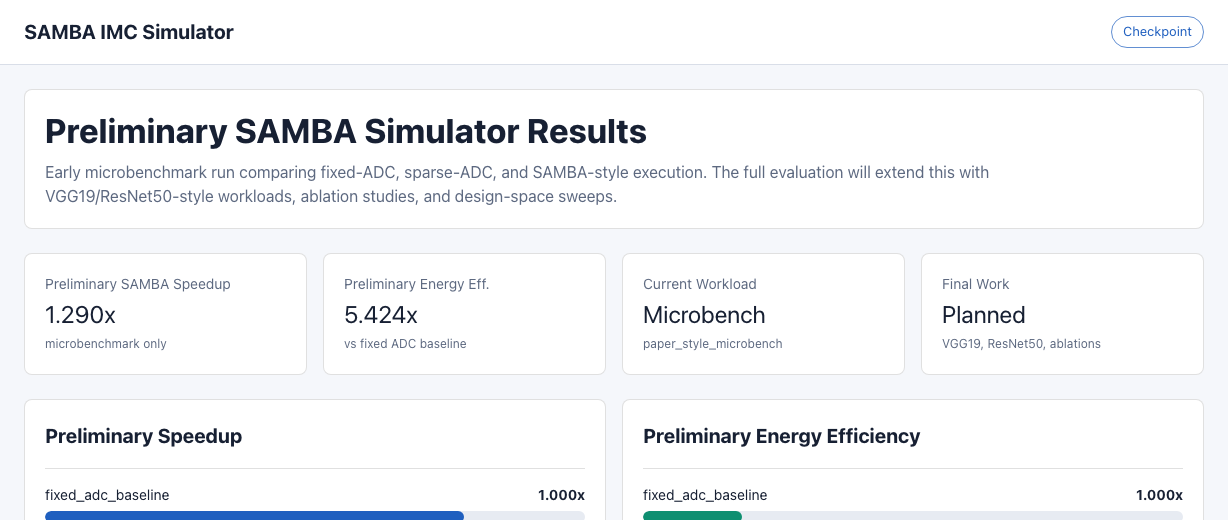
\includegraphics[width=0.92\textwidth]{docs/figures/proposal_dashboard_headline.png}
\caption{Current dashboard view for the preliminary SAMBA microbenchmark.}
\end{figure}

\section{Planned Final Results}

For the final presentation, I plan to show:

\begin{itemize}
    \item a complete fixed ADC vs sparse ADC vs SAMBA comparison,
    \item VGG19-style workload results,
    \item ResNet50-style workload results,
    \item ablation results for each SAMBA optimization,
    \item design-space sweep results,
    \item a React/Material UI dashboard,
    \item layer-level bottleneck analysis,
    \item trace-level evidence showing core and tile execution behavior.
\end{itemize}

The React/Material UI dashboard will be the main visual output for the final presentation. It will show metric cards, speedup charts, energy-efficiency charts, variant tables, and bottleneck-layer tables.

\section{Future Work}

The remaining work before the final presentation includes:

\begin{itemize}
    \item Complete the full ablation study for column exchange, row exchange, split MVMU, and data movement.
    \item Run VGG19-style and ResNet50-style experiments.
    \item Add more design-space sweeps for crossbar size, MVMUs per core, and cores per tile.
    \item Improve the simulator's overhead model for rearrange, load, store, send, receive, and ALU operations.
    \item Add final result charts and a Material UI dashboard.
    \item Add final validation tests and trace outputs.
    \item Prepare the final report and presentation slides.
\end{itemize}

A possible extension beyond this project would be to connect the simulator to real trained model weights from PyTorch or ONNX, or to export mappings into a lower-level hardware simulation framework.

\section{Team}

This is an individual project. I am responsible for reading the paper, designing the simulator, implementing the code, running experiments, analyzing results, writing the report, and preparing the final presentation.

\section{References}

\begin{enumerate}
    \item Dong Eun Kim, Aayush Ankit, Cheng Wang, and Kaushik Roy. ``SAMBA: Sparsity Aware In-Memory Computing Based Machine Learning Accelerator.'' \textit{IEEE Transactions on Computers}, 72(9), 2023.
    \item Aayush Ankit et al. ``PUMA: A Programmable Ultra-efficient Memristor-based Accelerator for Machine Learning Inference.'' \textit{ASPLOS}, 2019.
    \item Vivienne Sze, Yu-Hsin Chen, Tien-Ju Yang, and Joel S. Emer. ``Efficient Processing of Deep Neural Networks: A Tutorial and Survey.'' \textit{Proceedings of the IEEE}, 2017.
    \item Karen Simonyan and Andrew Zisserman. ``Very Deep Convolutional Networks for Large-Scale Image Recognition.'' \textit{ICLR}, 2015.
    \item Kaiming He, Xiangyu Zhang, Shaoqing Ren, and Jian Sun. ``Deep Residual Learning for Image Recognition.'' \textit{CVPR}, 2016.
    \item NumPy. \url{https://numpy.org/}
    \item Python. \url{https://www.python.org/}
    \item React. \url{https://react.dev/}
    \item Material UI. \url{https://mui.com/}
\end{enumerate}

\section{Source Code}

The proposal includes preliminary source code as required by the assignment. The current repository is available here:

\begin{center}
\texttt{https://github.com/Ashik20025/samba-imc-accelerator}
\end{center}

Important preliminary files include:

\begin{itemize}
    \item \texttt{src/samba/adc.py}: ADC precision, latency, and energy model.
    \item \texttt{src/samba/mapping.py}: Mapping layers to crossbar MVMUs.
    \item \texttt{src/samba/balancing.py}: Column exchange, row exchange, and split MVMU logic.
    \item \texttt{src/samba/simulator.py}: Experiment orchestration and simulation.
    \item \texttt{src/samba/reporting.py}: Report generation.
    \item \texttt{configs/microbench.json}: Preliminary microbenchmark configuration.
    \item \texttt{dashboard/}: Preliminary React/Material UI dashboard for proposal-stage visualization.
    \item \texttt{docs/figures/}: Preliminary dashboard screenshots for the proposal.
\end{itemize}

\subsection{Selected Preliminary Commands}

The following command runs the preliminary simulator:

\begin{lstlisting}
PYTHONPATH=src python3 -m samba run \
  --config configs/microbench.json \
  --out artifacts/microbench
\end{lstlisting}

The following command runs the preliminary test suite:

\begin{lstlisting}
PYTHONPATH=src python3 -m unittest discover -s tests
\end{lstlisting}

The final dashboard will be started locally using:

\begin{lstlisting}
./scripts/start_results_dashboard.sh
\end{lstlisting}

\end{document}
